%!TEX root = ../MasterThesis.tex

\section{Analysis of \gls{E-commerce} transactions}
\label{sec:analyse_transactions}

Based on the explanations in the previous section the idea is to link the transaction information from various merchants, \gls{LSP}s, \gls{PSP}s and issuers together into a shared information space to be able to analyse if there are any orders that look extraordinary, and are likely not being made by the owner of the credit card to a certain extend. Due to this proposal the collaborative system will also have to use statistical evaluations and probabilities to find and rate suspicious activities. Starting with the credit card in question an issuer can query for the order details of all the transactions that have been done with the credit card online recently. To be able to do that an issuer will likely have to query the \gls{PSP}s for the payment tokens first, before asking the affected merchants for order details to any of those payment tokens. At the end each online transaction can be mapped into an \gls{ER} model like the one shown in Figure~\ref{fig:images_data_model}, building up a large graph of entities and their relationships, which has the specific credit card in the centre of it. An abbreviated sample graph of this procedure can be seen in Figure~\ref{fig:images_credit_card_graph}. \@

\begin{figure}[H]
  \centering
  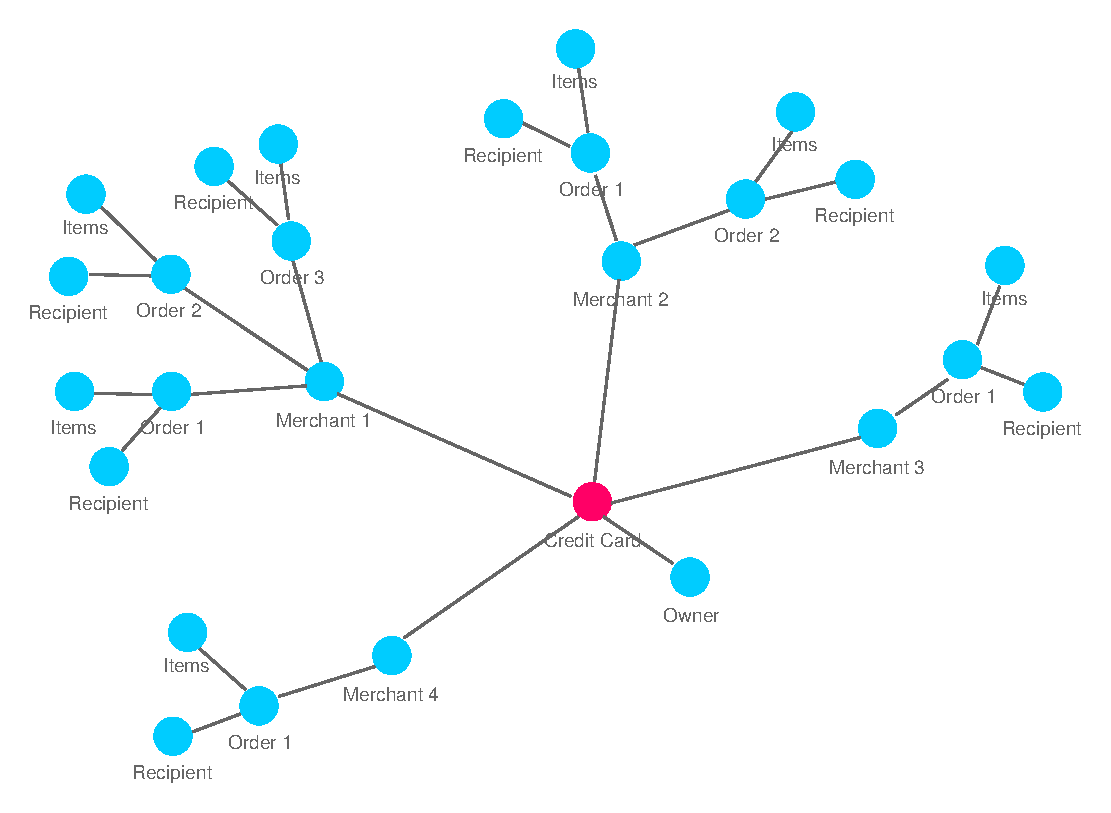
\includegraphics[width=0.9\columnwidth]{images/ontology_scenario_2.pdf}
  \caption{Building clusters of \gls{E-commerce} transactions by merchant}
\label{fig:images_credit_card_graph}
\end{figure}

As shown in this figure the transactions will be clustered by merchants first. But collecting the various order information into one combined data set is just the beginning of the \gls{E-commerce} fraud incident analysis. Based on the information received an issuer can already filter out transactions that have been shipped to different addresses than the one the credit card owner is registered for. Particularly for those edge cases it might be worth to ask for additional information from the affected merchants to be able to figure out if the consumer has used one of these shipping addresses before. As a result the existing data set can be further enriched with supplementary transactional information from merchants at any time if needed. In addition to the address information an issuer can also analyse the item information (\gls{incl}\ category, brand and model) of each order to check for malicious activities. \\

But as already stated analysing the cluster of transactions on a merchant by merchant basis will not be sufficient to come up with a solid decision about a suspicious transaction. This is mostly due to the usage pattern of the fraudsters that have been explained in the scenario in Section~\ref{sec:scope_thesis}. Based on this description the various order details from the merchants have to be mapped and linked against each other, so that the initial graph of transactions, which is clustered by merchant, can be easily transformed into complementary representations, which use different criteria to cluster the transactions such as recipient addresses, branches of merchants, or product-related information. \\

This reshaping of the transactional details can lead to new insights about the ``normal'' shopping behaviour of a credit card owner, and can make deviations from this behaviour visible. By using a clustered graph to visualize the combined data set on screen the exploratory nature of knowledge generation and perception will be supported, and so this kind of representation can help speed up the investigation of \gls{E-commerce} fraud incidents. An example visualization of a clustered graph, which groups information together based on a chosen criteria, is depicted in Figure~\ref{fig:images_graph_viz}. The different colours in this figure can represent different sources of information (e.g.\ \gls{E-commerce} transactions from various merchants). In this example information that stands out from the ``normal behaviour'' can be found in the top right and lower left areas of the figure. \@

\begin{figure}[H]
  \centering
  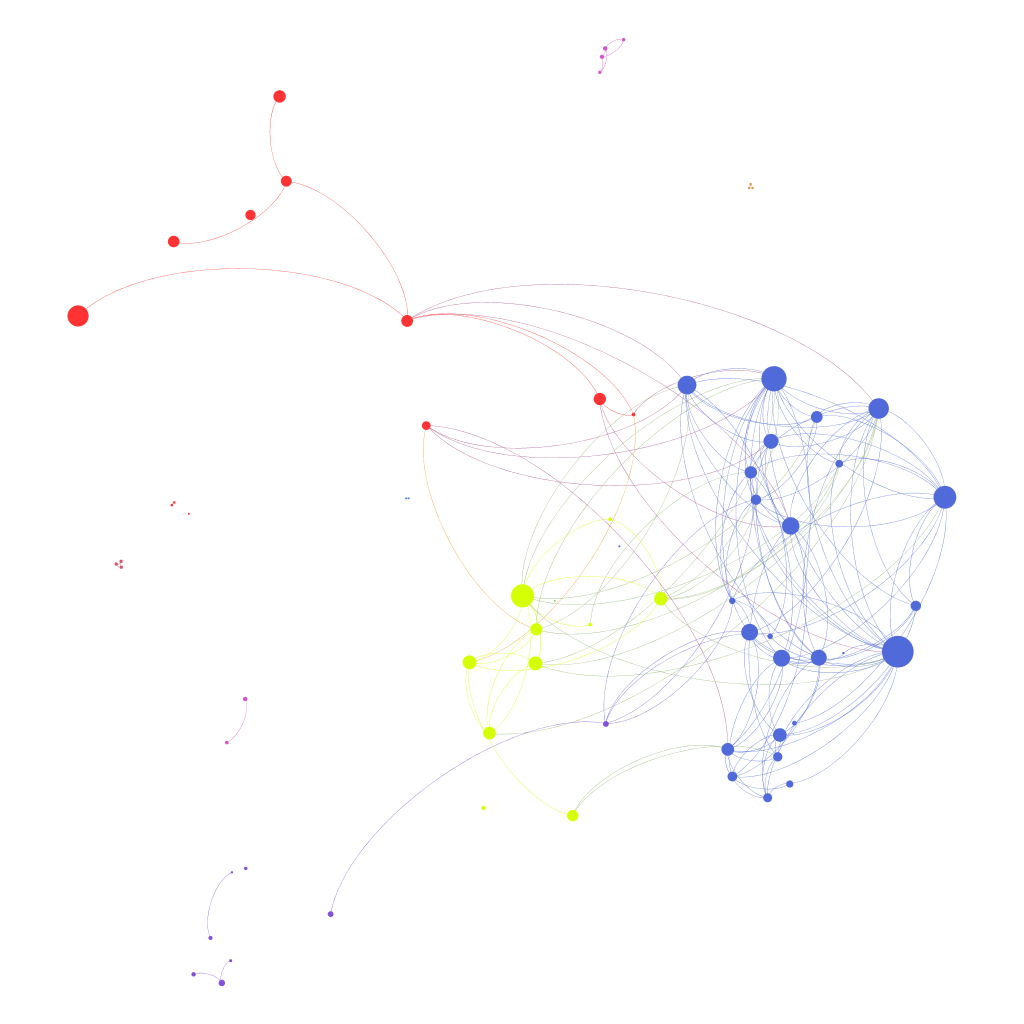
\includegraphics[width=0.8\columnwidth]{images/GraphViz.png}
  \caption[An example visualization of a clustered graph]{An example visualization of a clustered graph \citep{griffsgraphs}}
\label{fig:images_graph_viz}
\end{figure}

 In addition to these clustered graph visualizations the collaborative system can also support the \gls{E-commerce} fraud investigation by switching the type of representation based on the chosen criteria; e.g.\ when clustering transaction details based on location information such as shipping addresses the system can present the information as a heat map on a chart as is displayed in Figure~\ref{fig:images_map_heatmap}. \@

\begin{figure}[H]
  \centering
  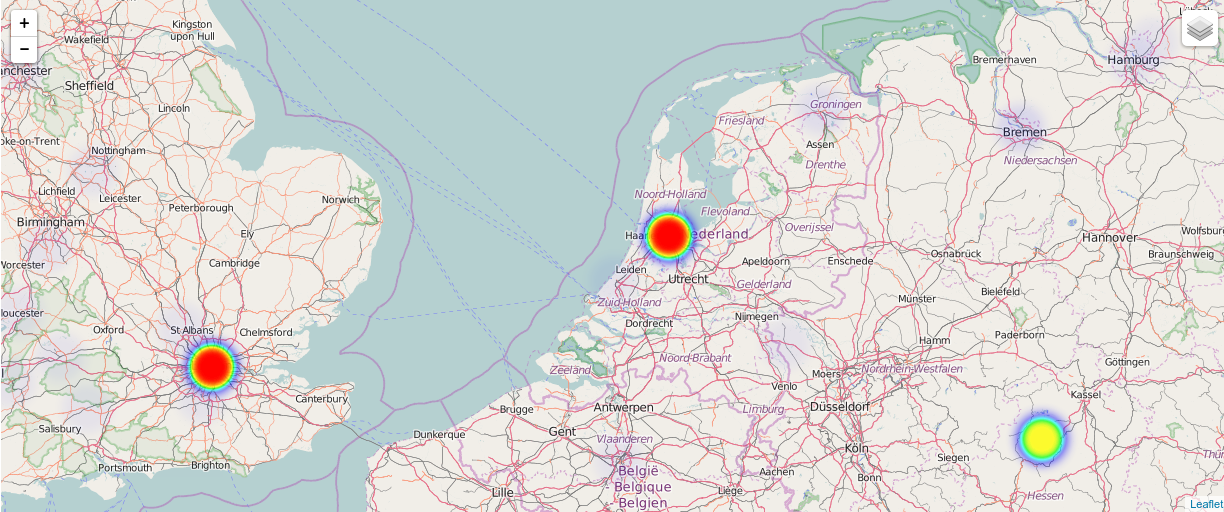
\includegraphics[width=0.9\columnwidth]{images/Heatmap.png}
  \caption{Heatmap displaying clusters of location-based information}
\label{fig:images_map_heatmap}
\end{figure}

Additionally, the collaborative system can provide a Hypertext-based visualization of the linked information to allow investigators navigating through the consolidated order details done with a credit card recently. \\

To conclude the system have to support the collection and combination of \gls{E-commerce} transaction information from various sources into a linked data set using a graph-oriented data model. This graph can further be analysed from multiple view points to validate if there are any transactions that stand out from the ``normal'' shopping behaviour of the credit card owner. The starting point for the investigation is a sequence of payment tokens of recent credit card activities that an issuer can provide to the \gls{PSP}s. The linked data set will initially collect and cluster the information from each merchant based on this list. In case there are already suspicious information in one of these clusters, an issuer can ask for further details and enrich that specific cluster with additional order information for this consumer and that merchant. In the final step the system has to do the mapping and linking of the order detail information between each merchant to allow subsequent analysing and clustering of the transaction details based on various criteria, see Figure~\ref{fig:system_workflow}.

\begin{figure}[H]
  \centering
  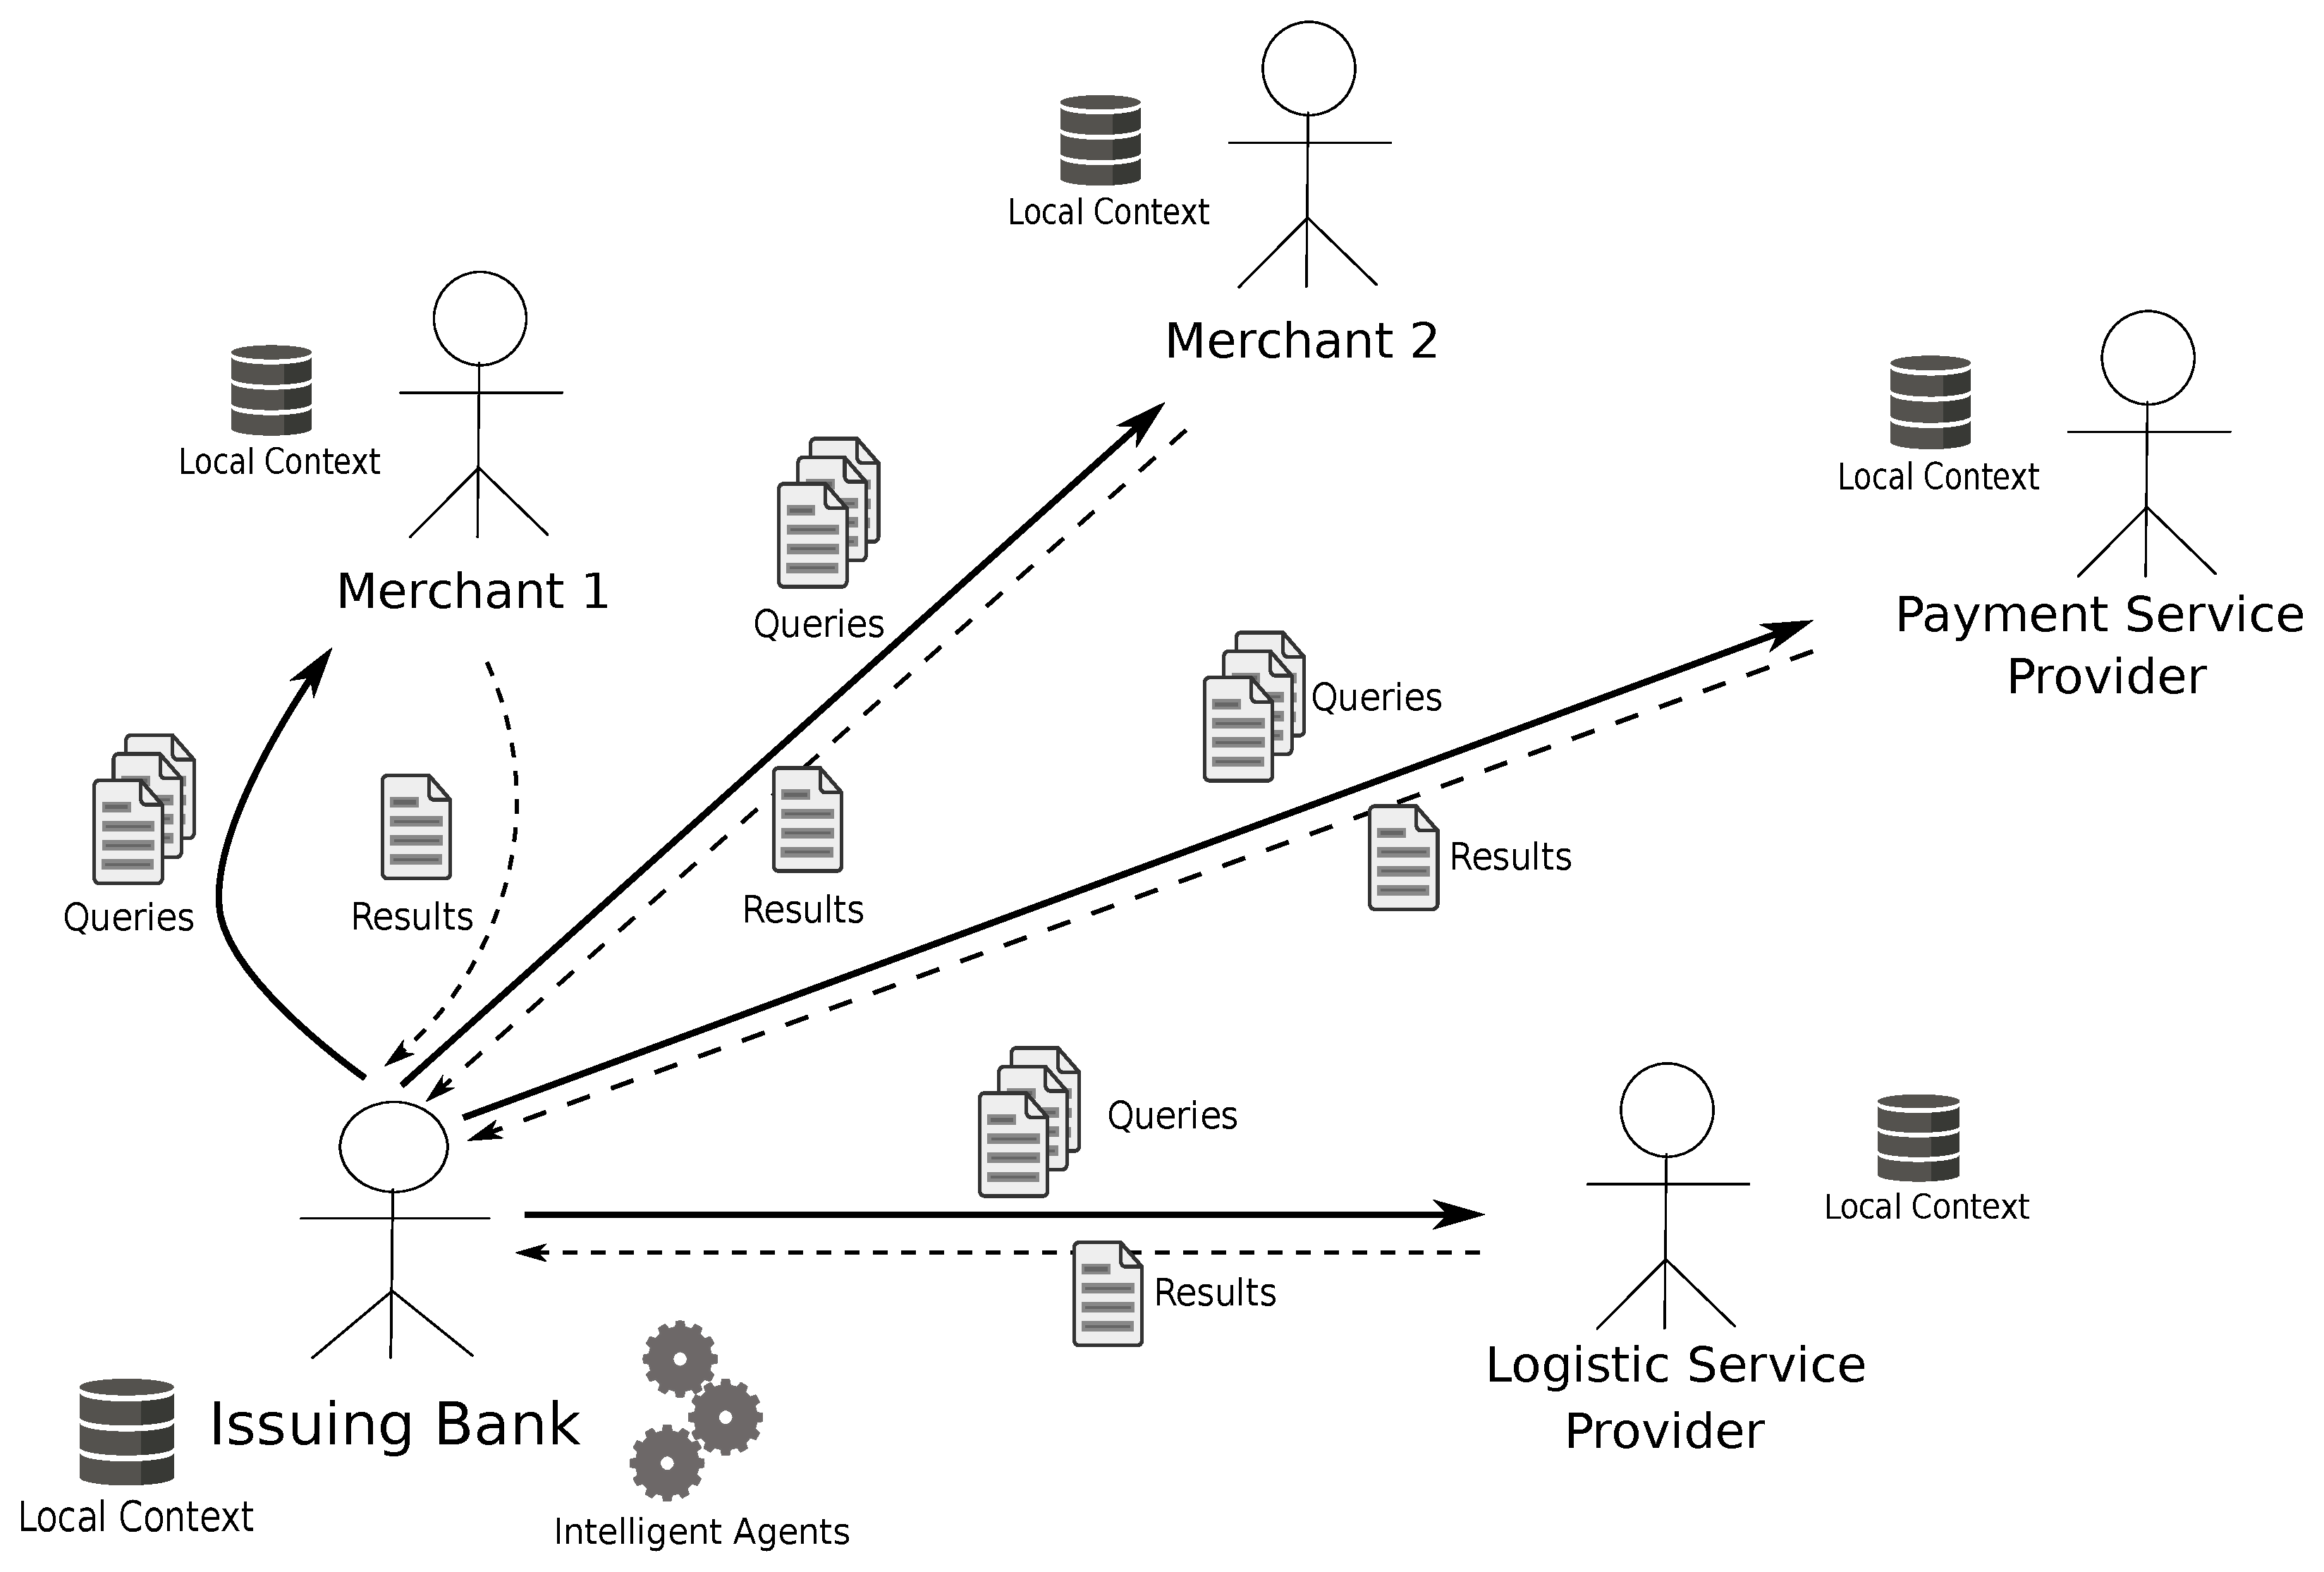
\includegraphics[width=0.7\columnwidth]{images/system_P2P_decentralized.pdf}
  \caption{Information flow in the proposed collaborative system}
\label{fig:system_workflow}
\end{figure}

% section system_overview (end)
